%=====================================================================
\section{How long may fault detection take? (RQ2, empirical)}\label{sec:delay}
%=====================================================================
\subsection{The failure timeline}
Figure~\ref{fig:timeline} shows what happens around a failure. At $t=0$ rotor 4 stops. The flight computer does not know this yet, so the healthy controller keeps flying. At $t=\tau$ (the \emph{detection delay}) a detector raises the alarm and a supervisor switches to the failure-mode strategy, which must \emph{capture} the drone into the relaxed hover from wherever it has drifted.

\begin{figure}[h]
\centering
\begin{tikzpicture}[>=Stealth, box/.style={draw, rounded corners=2pt, align=center, minimum height=1.25cm, text width=2.35cm, font=\small}]
  \node[box, fill=gray!8] (a) {Healthy flight\\ \scriptsize 4 rotors, healthy LQR};
  \node[box, fill=gray!8, right=0.45cm of a] (b) {Rotor fails\\ \scriptsize $t = 0$};
  \node[box, fill=orange!12, draw=orange!70!black, right=0.45cm of b] (c) {Undetected\\ \scriptsize healthy LQR flies a 3-rotor drone for $\tau$};
  \node[box, fill=gray!8, right=0.45cm of c] (d) {Capture\\ \scriptsize spin-up, then failure controller};
  \node[box, fill=blue!8, right=0.45cm of d] (e) {Relaxed hover\\ \scriptsize steady spin};
  \foreach \u/\v in {a/b,b/c,c/d,d/e} \draw[->,thick] (\u) -- (\v);
\end{tikzpicture}
\caption{The failure timeline. RQ2 is about the orange phase: how long it may last.}\label{fig:timeline}
\end{figure}

\subsection{Why the undetected phase is dangerous: a simple bound}
Right after the failure the drone is still near level hover, so the body rates are small and the gyroscopic terms in~\eqref{eq:rot} are negligible. The roll equation then reduces to
\begin{equation}
  I^B_{xx}\,\dot p = l\,(f_2 - f_4) = l\,f_2,
\end{equation}
because $f_4 = 0$. Rotor 2, opposite the failed rotor, now pushes one side up with nothing to balance it. The healthy controller notices the roll and reduces $f_2$, but it keeps its motors running, and a running motor cannot go below its idle thrust $f_{\min}$. Hence
\begin{equation}
  \dot p \;\ge\; \frac{l\,f_{\min}}{I^B_{xx}} = \frac{0.17\times0.2}{3.2\times10^{-3}} = 10.6\ \text{rad/s}^2 .
\end{equation}
This holds for \emph{any} healthy controller whose motor allocation keeps running motors at or above idle, as standard autopilots do, however it is tuned. Integrating twice gives a lower bound on the roll angle, $\tfrac12(lf_{\min}/I^B_{xx})t^2$.

Figure~\ref{fig:undetected} shows the simulation for three tunings of the healthy LQR ($\alpha = 0.3$, 1 and 3): the tilt reaches about 12 to 15$^\circ$ at 100\,ms and 33 to 43$^\circ$ at 200\,ms, so a more aggressive tuning helps only a little. Rotor 2's thrust falls close to its idle limit within about 100\,ms; the controller then has no roll authority left.

\begin{figure}[h]
\centering
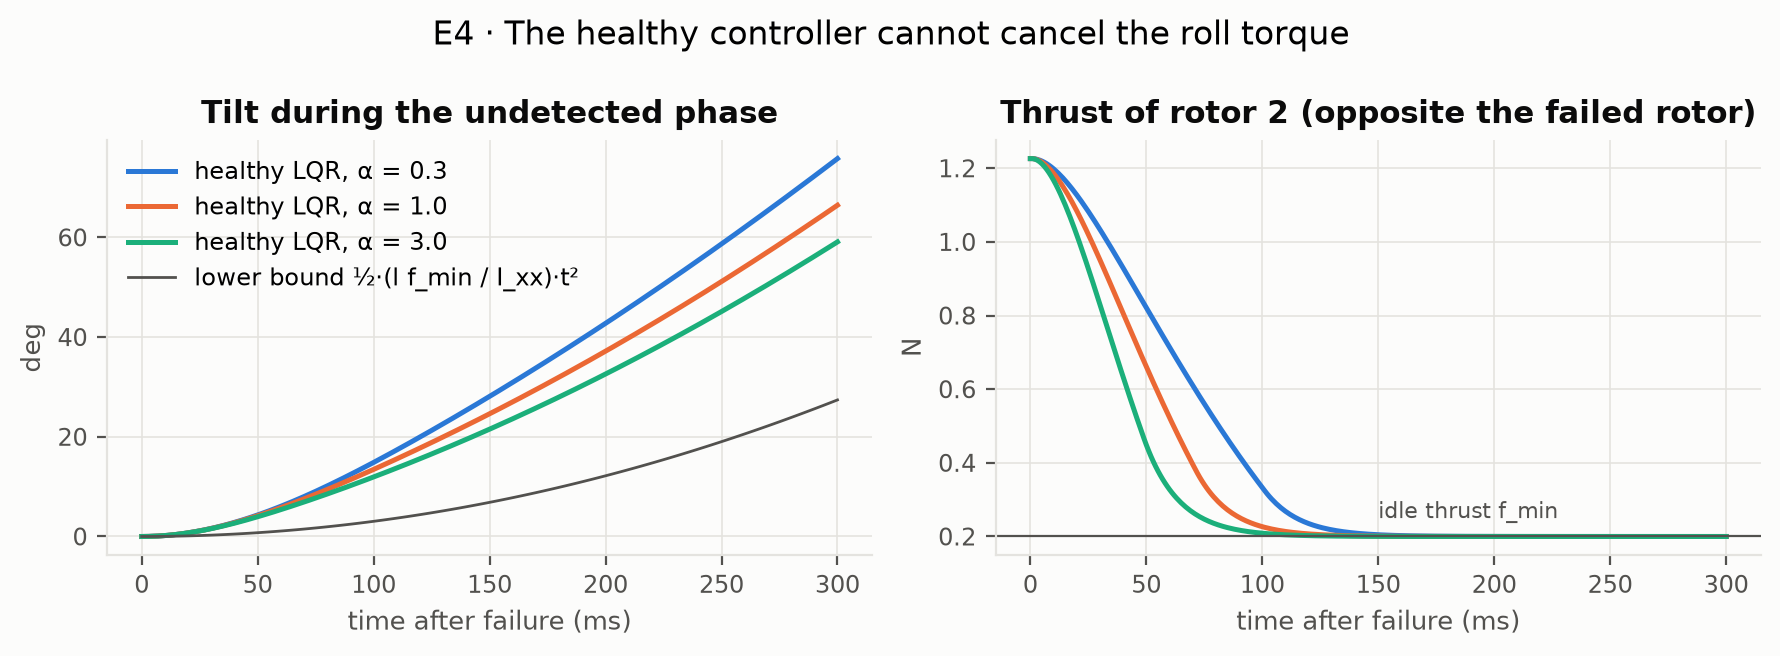
\includegraphics[width=\linewidth]{figures/e4_undetected_phase.png}
\caption{Undetected phase. Left: tilt for three healthy-controller tunings with the analytic lower bound. Right: thrust of rotor 2, which drops to idle.}\label{fig:undetected}
\end{figure}

\subsection{Experimental design (E4)}
\paragraph{Scenario.} The drone hovers at height 0 on the nominal plant. At $t=0$ rotor 4 fails. Until $t=\tau$ the healthy LQR flies (its command to rotor 4 has no effect). At $t=\tau$ a supervisor switches to one of these failure strategies:
\begin{itemize}
  \item \textbf{Direct LQR}: the failure LQR is switched on at once.
  \item \textbf{Spin-up, then LQR} (the strategy of~\cite{mueller2014stability}, used in their flight; the details below are read from their Fig.~4): rotors 1 and 3 run at a fixed thrust $f_{\text{spin}}$, rotor 2 is stopped, with no attitude feedback, until the rotation rate exceeds 10\,rad/s; then the failure LQR takes over. We use $f_{\text{spin}} = 2.95$\,N (read from the flight data) and, as a sensitivity case, $mg/2 = 2.45$\,N.
\end{itemize}
At the switch, the failure controller's motor-thrust estimate is initialized from the supervisor's filter of the commands it sent before, never from the true thrust. Each run lasts 10\,s, with the controller at 1\,ms.

\begin{codebox}{the detection-delay supervisor}
\begin{lstlisting}
def alive(self, t):                     # which rotors produce thrust
    return np.array([True, True, True, t < self.t_fail])

def __call__(self, t, x):
    if t < self.t_fail + self.tau:      # failure not yet detected
        u = self.healthy(t, x)          # (also updates a filter of the commands sent)
        return u
    if not self.switched:               # first call after detection
        self.failure.reset(self.f_cmd_est)
        self.switched = True
    return self.failure(t, x)           # spin-up, then failure LQR
\end{lstlisting}
\end{codebox}

\paragraph{Success criterion, fixed before the runs.} It is written in \texttt{metrics.py} and was not changed after seeing results. A run is
\begin{itemize}
  \item \textbf{captured} if, over the last 1\,s of a run that did not stop early, the reduced attitude is within 0.05 of $\bar{\vect n}$ and the body rates are within 2\,rad/s of $\bar{\vect\omega}$;
  \item \textbf{safe} if it is captured, \emph{and} the height loss (starting height minus lowest height) is below 2\,m, \emph{and} the drone never turns upside down ($n_z > 0$ throughout).
\end{itemize}

\paragraph{Monte Carlo.} A real failure does not happen at a perfect hover. For each delay $\tau = 0, 5, 10, \dots, 60$\,ms and each spin-up thrust we ran 40 simulations from random pre-failure states (velocity with standard deviation 0.3\,m/s, Euler angles 3$^\circ$, body rates 0.3\,rad/s; the same 40 seeds for every delay). The estimated probability of a safe recovery is $\hat p = k/n$ ($k$ safe runs out of $n=40$). Its 95\% \emph{Wilson} confidence interval is
\begin{equation}
  c \pm h, \qquad c = \frac{\hat p + z^2/(2n)}{1+z^2/n}, \qquad h = \frac{z}{1+z^2/n}\sqrt{\frac{\hat p(1-\hat p)}{n} + \frac{z^2}{4n^2}}, \qquad z = 1.96 .
\end{equation}
Unlike the textbook interval $\hat p \pm z\sqrt{\hat p(1-\hat p)/n}$, it does not collapse to zero width when $\hat p$ is 0 or 1. We summarize each curve by $\tau_{90}$ and $\tau_{50}$, the delays at which $\hat p$ first falls below 0.9 and 0.5 (linear interpolation between grid points). We also swept $\tau$ from 0 to 300\,ms in 10\,ms steps from the exact hover, for all three strategies, and for three healthy-controller tunings with the 2.95\,N spin-up.

\subsection{Results}
\begin{table}[h]
\centering\footnotesize
\caption{Spin-up then LQR: fraction of safe recoveries in 40 random starts per delay, with 95\% Wilson intervals.}\label{tab:delay}
\setlength{\tabcolsep}{3pt}
\begin{tabular}{lccccccc}
\toprule
Delay $\tau$ & 0\,ms & 5\,ms & 10\,ms & 15\,ms & 20\,ms & 30\,ms & 40\,ms \\
\midrule
2.95\,N & 1.00 & 1.00 & 0.97 & 0.80 & 0.42 & 0.17 & 0.07 \\
 & [0.91, 1] & [0.91, 1] & [0.87, 1] & [0.65, 0.90] & [0.29, 0.58] & [0.09, 0.32] & [0.03, 0.20] \\
\midrule
2.45\,N & 1.00 & 0.95 & 0.82 & 0.45 & 0.28 & 0.07 & 0.07 \\
 & [0.91, 1] & [0.83, 0.99] & [0.68, 0.91] & [0.31, 0.60] & [0.16, 0.43] & [0.03, 0.20] & [0.03, 0.20] \\
\bottomrule
\end{tabular}
\end{table}

\begin{figure}[h]
\centering
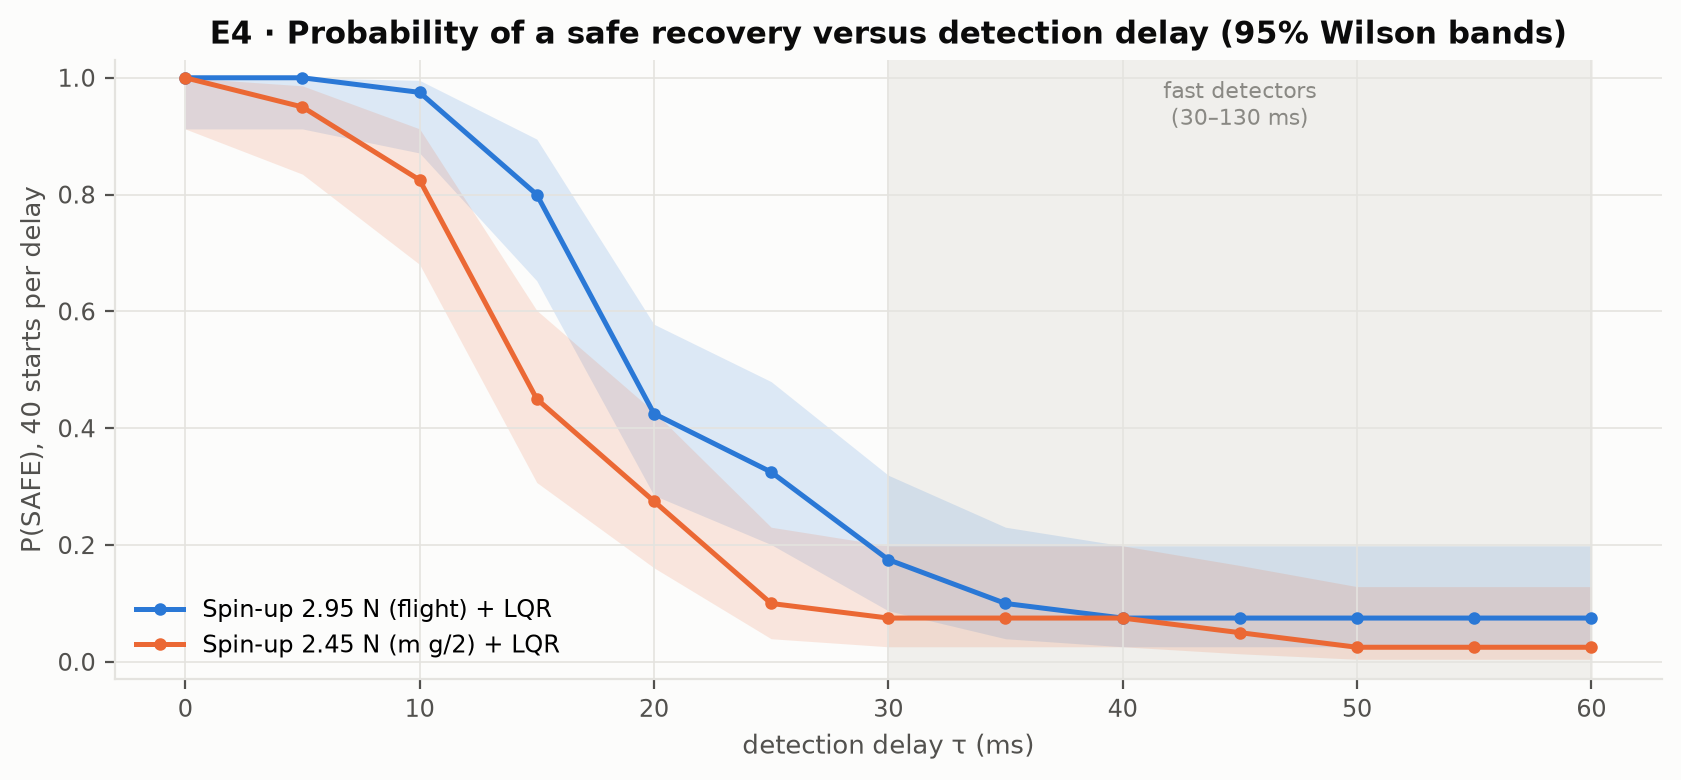
\includegraphics[width=0.85\linewidth]{figures/e4_p_safe.png}
\caption{Probability of a safe recovery against detection delay for the two spin-up thrusts, with 95\% Wilson bands. The shaded region marks the 30 to 130\,ms reported for one fast detector~\cite{strack2021fast}.}\label{fig:psafe}
\end{figure}

\paragraph{Main result.} With the flight spin-up thrust, the probability of a safe recovery falls below 0.9 at about \textbf{12\,ms} of delay and below 0.5 at about \textbf{19\,ms} (Table~\ref{tab:delay}, Figure~\ref{fig:psafe}). With the lower thrust $mg/2$ these are 7 and 14\,ms. If only attitude capture is required (ignoring height loss), the 50\% point moves to 52\,ms (40\,ms with $mg/2$). Published detectors need about 20 to 130\,ms~\cite{strack2021fast,yang2026mml1,zhou2025rotorfailureaware}, so with this strategy a safe recovery is unlikely within the time most current detectors need.

\paragraph{No delay matches the flight.} With the flight thrust and $\tau = 0$, the drone first climbs 0.40\,m and then drops only 0.03\,m below its starting height, qualitatively like the real flight, which climbed about 0.9\,m.

\paragraph{Direct LQR fails.} Switching the failure LQR on directly, without spin-up, captures the attitude in the end but always turns the drone upside down on the way and loses 9 to 16\,m of height, at every delay (Figure~\ref{fig:sweep}). The LQR was designed for a drone that already spins at 19\,rad/s; right after the failure the drone does not spin yet, and the linear model is far from valid there. Section~\ref{sec:certificate} returns to this point.

\begin{figure}[h]
\centering
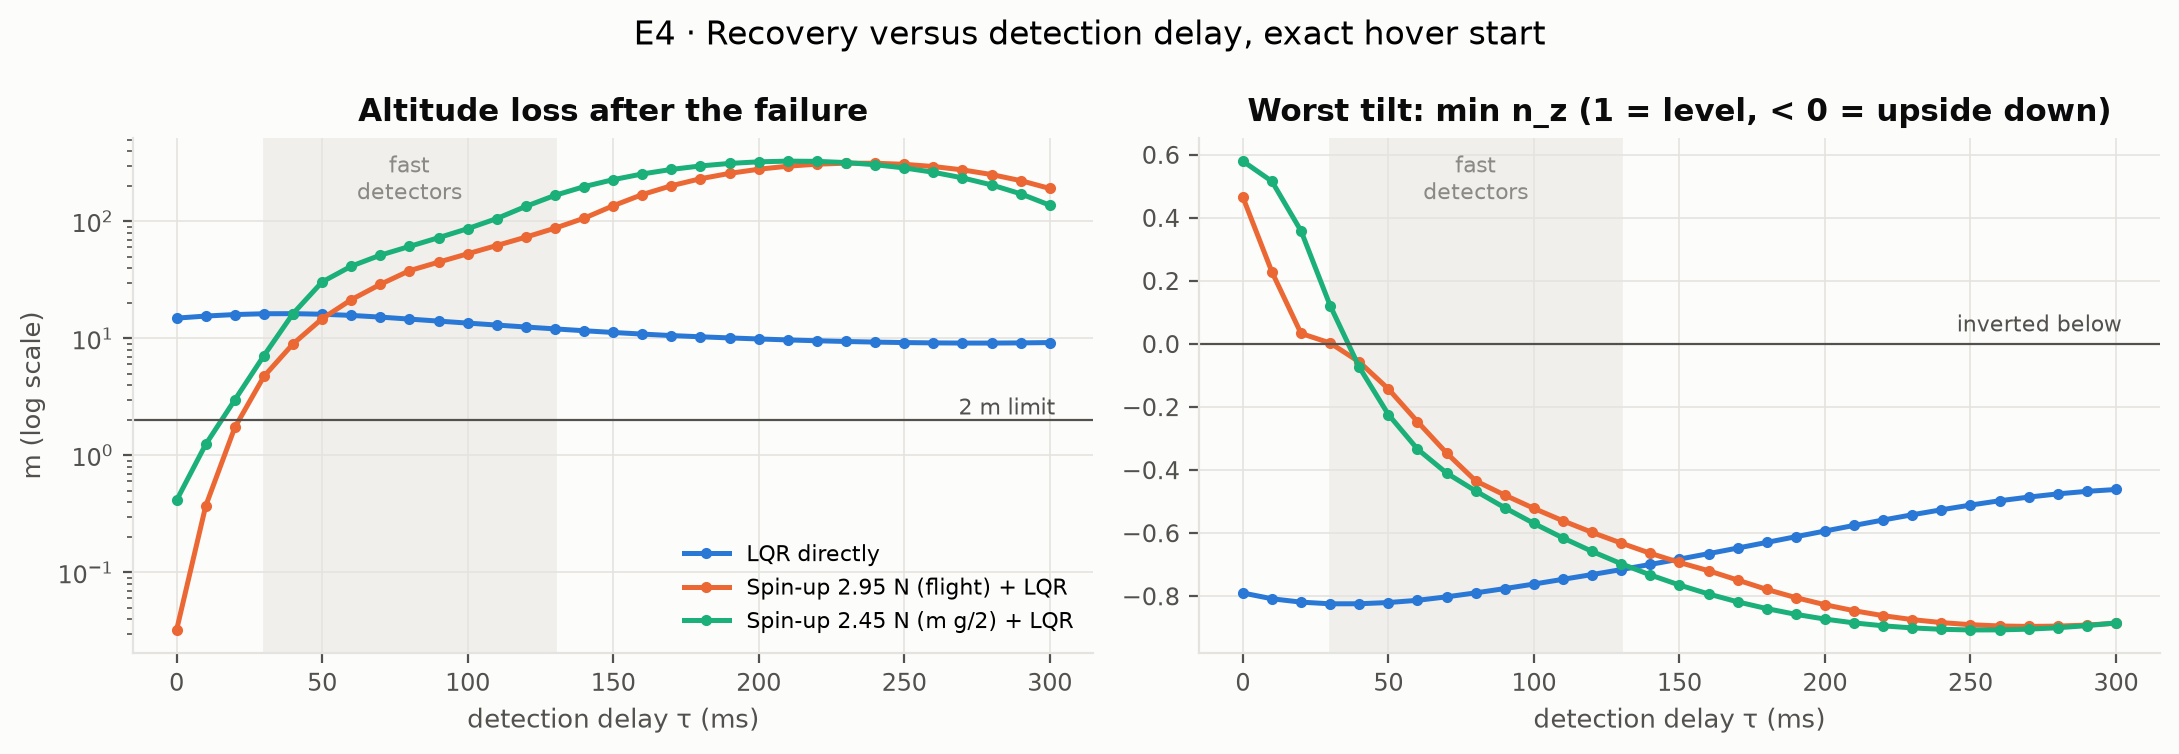
\includegraphics[width=\linewidth]{figures/e4_delay_sweep.png}
\caption{Exact hover start, delays 0 to 300\,ms. Left: height loss (log scale) with the 2\,m limit. Right: the worst tilt, $\min n_z$ (below 0 means upside down).}\label{fig:sweep}
\end{figure}

\begin{figure}[h]
\centering
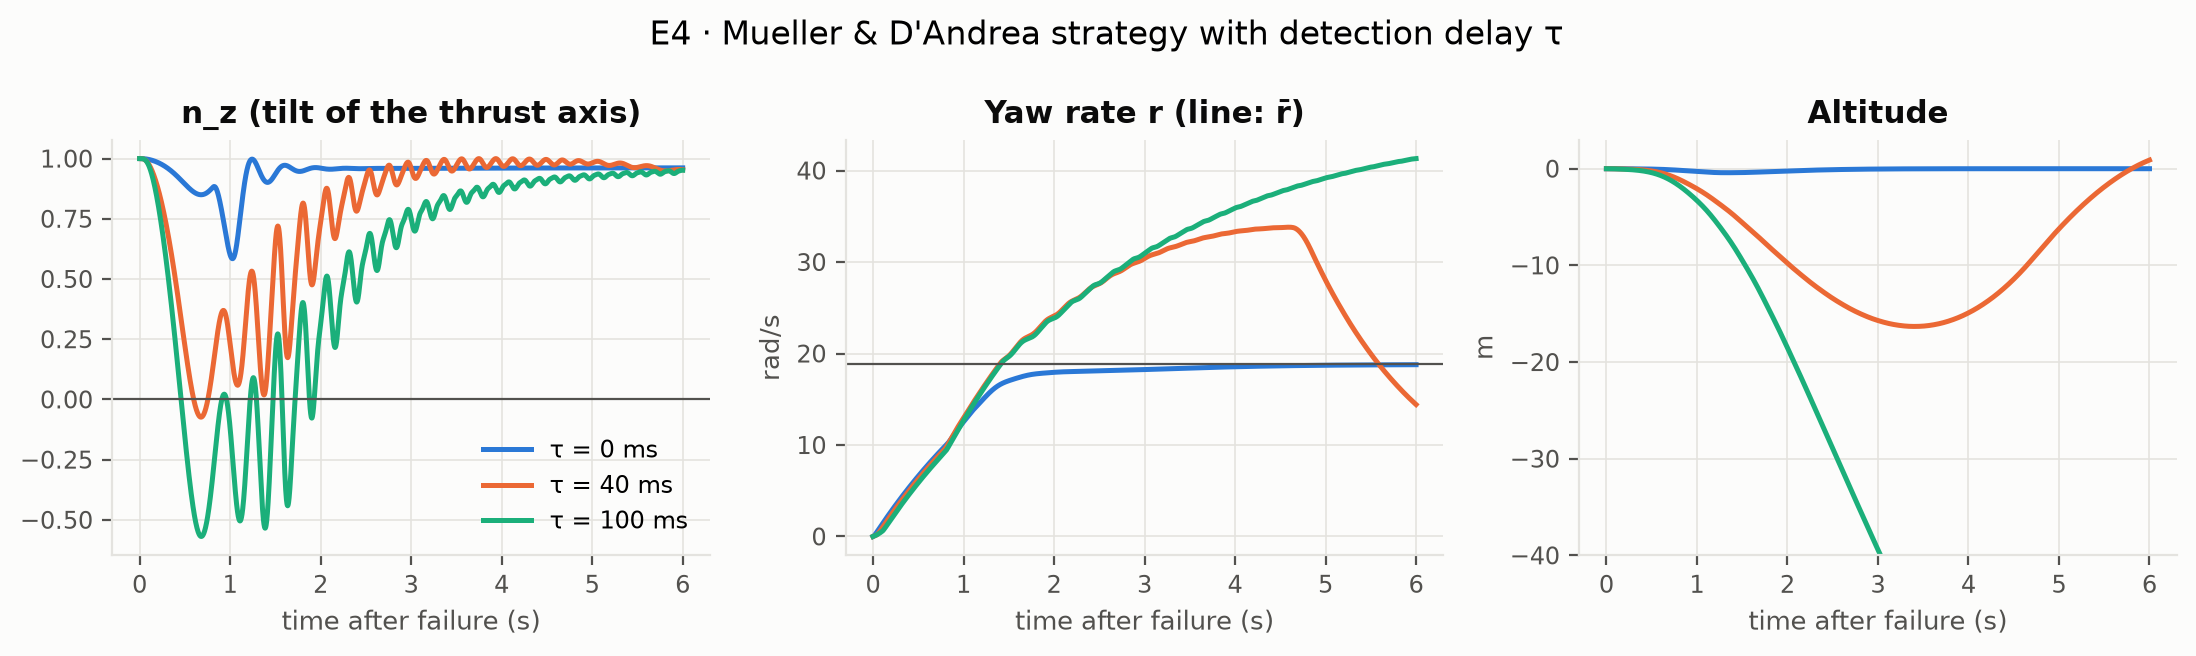
\includegraphics[width=\linewidth]{figures/e4_time_histories.png}
\caption{Spin-up (2.95\,N) then LQR for delays of 0, 20 and 50\,ms: tilt, yaw rate and height.}\label{fig:histories}
\end{figure}

\paragraph{Tuning does not help.} From the exact hover start, every delay up to 20\,ms is safe for all three healthy-controller tunings ($\alpha = 0.3$, 1, 3), and 30\,ms is not. This agrees with the idle-thrust bound: no tuning can stop the roll.

\paragraph{Scope.} These numbers belong to this strategy and this model. In other simulation studies, nonlinear controllers recovered, with some loss of performance, at detection delays of about 0.1 to 0.2\,s~\cite{chen2025learning,zhou2025rotorfailureaware}, so the limit is not a property of rotor loss in general.

\subsection{Do the MPCs tolerate more delay?}
RQ2 asks how the capture controller changes the tolerable delay. As a first look we repeated the scenario on truth plant A with each controller of Section~\ref{sec:mpc} as the capture controller (spin-up at 2.95\,N, then LQR, analytical MPC or residual Koopman MPC). On a mismatched plant a controller designed on the nominal model settles at its own steady state, not at the plant's equilibrium, so capture was judged against each controller's own steady state (found by a 12\,s run from the trim).

\begin{center}\small
\begin{tabular}{lccc}
\toprule
$\tau$ & LQR & MPC, analytical & MPC, residual Koopman \\
\midrule
0\,ms & safe (0.40\,m) & safe (0.53\,m) & safe (0.58\,m) \\
10\,ms & safe (1.69\,m) & inverted (2.52\,m) & inverted (2.80\,m) \\
20\,ms & inverted (6.56\,m) & inverted (8.53\,m) & inverted (7.94\,m) \\
\bottomrule
\end{tabular}
\end{center}
(Height loss in brackets; one run per entry.) LQR is safe up to 10\,ms, both MPCs only without delay. We do not yet understand why. The LQR uses the same linear model and weights, so model validity alone does not explain the difference; candidates are the short 100\,ms horizon and the thrust limits becoming active during capture, where the MPC and the clipped LQR act differently. (All three controllers run at 5\,ms in this comparison.) This needs further study. Note that this table uses plant A and a 5\,ms sample period for every controller (including the healthy one), while Table~\ref{tab:delay} uses the nominal plant and 1\,ms; slower sampling alone adds effective delay, so their absolute numbers are not directly comparable.
